\begin{Ueberlieferung}% 
{\textit{L}}Aufzeichnung: LH XXXVII 5 Bl. 139. 1 Bl. 4\textsuperscript{o}. \unitfrac{3}{4} S. auf Bl. 139 r\textsuperscript{o}. Bl. 139 v\textsuperscript{o} leer. Texttr\"{a}ger durch Papiererhaltungsma{\ss}nahmen gesichert. \\ Cc 2, Nr. 943
\end{Ueberlieferung}

\count\Bfootins=1200
\pstartfirst 
[139~r\textsuperscript{o}] April. 1675.\pend 
\pstart \noindent
Si motus\protect\index{Sachverzeichnis}{motus} nil nisi relativum est, sequitur eosdem esse effectus\protect\index{Sachverzeichnis}{effectus} concursuum\protect\index{Sachverzeichnis}{concursuum} sive corpora\protect\index{Sachverzeichnis}{corpora} \edtext{\textit{A} et \textit{B} concurrant}{\lemma{}\Bfootnote{\textit{A} et \textit{B} \textbar\ aequali celeritate \textit{gestr.}\ \textbar\ concurrant \textit{L}}}
in ((\textit{A}))((\textit{B})), sive in (((\textit{A})))\textit{B}. Id est nulla erit differentia inter effectus celeritatis absolutae\protect\index{Sachverzeichnis}{celeritas!absoluta} ac respectivae\protect\index{Sachverzeichnis}{?}; adeoque idem eveniet sive duo corpora  aequalia \textit{A} et \textit{B} aequali celeritate in eadem recta sibi in medio itineris occurrant sive contra uno ex illis quiescente, alterum dupla celeritate latum intelligatur. Quod experientiae\protect\index{Sachverzeichnis}{experientia} contrarium est, nam si sint corpora Elaterio\protect\index{Sachverzeichnis}{elaterium} carentia priori modo quiescent ambo, posteriore servato ipsius \textit{A} motu, \textit{B} posterius cum eo abripietur. Sed et calculus
\edtext{ostendit in Elasticis,}{\lemma{ostendit}\Bfootnote{\textit{(1)}\ , jungendos esse calculos duos impetus\protect\index{Sachverzeichnis}{impetus} impressi \textit{(2)}\ in Elasticis, \textit{L}\hspace{-2mm}}}
non tantum ictus a respectiva celeritate, seu appropinquatione ac collisione corporum, sed et ipsius absoluti motus habendam esse rationem. Nam alioquin Elastica\protect\index{Sachverzeichnis}{Elasticum} post concursum eodem resilirent modo, quaecunque fuisset celeritas alterutrius, modo eadem fuisset \edtext{appropinquationis quantitas}{\lemma{fuisset}\Bfootnote{\textit{(1)}\ celeri \textit{(2)}\ motus summa \textit{(3)}\ appropinquationis quantitas, \textit{L}\hspace{-2mm}}}, quod experientiae adversatur. \edtext{Si}{\lemma{adversatur.}\Bfootnote{\textit{(1)}\ Celeritas corpori impellentis, communicatur \textit{(2)}\ Si \textit{L}\hspace{-2mm}}} concursus motuum satis compositionibus explicari possent sequeretur corpus magnum aeque facile impelli ac parvum. Cum contra compertum \edtext{sit, [eundem] esse non quidem gradum, attamen quantitatem motus.%
}{\lemma{sit,}\Bfootnote{%
\textit{(1)}~eandem esse non quidem quantitatem celeritatis, sed motus %
\textit{(2)}~eandem [...] motus \textit{L ändert Hrsg.}}} Quae omnia probant corpora non seipsis sed circumfusae materiae fluctibus ferri, ut fit in illis quae liquido innatant.
\pend
\vspace{2em}
\pstart
\centering 
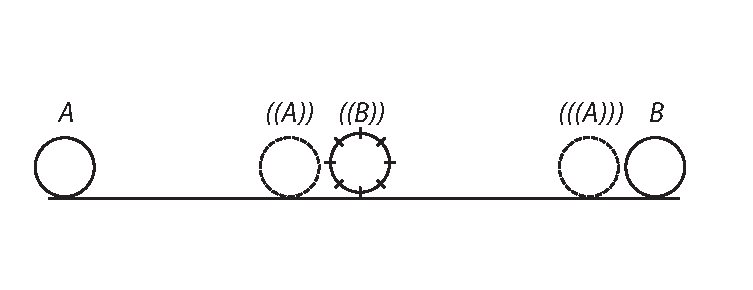
\includegraphics[trim = 0mm -3mm 0mm 0mm, clip, width=0.6\textwidth]{images/lh03705139r}\\
 \noindent \centering [\textit{Fig. 1}] 
%\caption{Bildbeschreibung}
\pend
\newpage
\count\Bfootins=1200
\pstart Funiculum ex arena necti per motum, sive Motum esse principium cohaesionis\protect\index{Sachverzeichnis}{cohaesio} in rebus duobus inprimis experimentis apparet Magnete\protect\index{Sachverzeichnis}{magnes}, et jactibus aquarum aliorumque fluidorum. Nam si \edtext{chalybis}{\lemma{si}\Bfootnote{\textit{(1)}\ filamenta \textit{(2)}\ chalybis \textit{L}}} scobem \edtext{chartae inspersam}{\lemma{}\Bfootnote{chartae inspersam \textit{erg.} \textit{L}}} magneti admoveas, senties \edtext{pilos}{\lemma{senties}\Bfootnote{\textit{(1)}\ capillos \textit{(2)}\ pilos \textit{L}}} quasi quosdam formari ex promotu chartae, instar \edtext{acicularum erinacei erigi}{\lemma{instar}\Bfootnote{\textit{(1)}\ erina \textit{(2)}\ pili erinacei erigi \textit{(3)}\ acicularum erinacei erigi. \textit{L}}}. Ablato magnete rursus in pulverem concidunt. Unde facile judicari potest motu fieri eorum cohaesionem, quid enim aliud contribuat magnes. Quod attinet jactus aquarum, patet non nisi motu formari \edtext{ex liquido}{\lemma{formari}\Bfootnote{\textit{(1)}\ ex aere \textit{(2)}\ ex liquido \textit{L}}} solidi cujusdam corporis \edtext{imitationem. Et experimentum}{\lemma{imitationem.}\Bfootnote{\textit{(1)}\ Idque \textit{(2)}\ Et \textbar\ motu corporum \textit{gestr.} \textbar\ experimentum \textit{L}}}
rei capi potest;
\edtext{manu perfora}{\lemma{manu perfora}\Bfootnote{\textit{erg. L}}}
\edtext{[vel]}{\lemma{vel}\Bfootnote{\textit{erg. Hrsg.}}}
trajice sagitta aut lapide jactum aquae, eodem trajice ejusdem crassitiei\protect\index{Sachverzeichnis}{crassitieis} aquam quiescentem, senties minorem resistentiam\protect\index{Sachverzeichnis}{resistentia} in quiescente. Sed unum hic considerandum videtur, motum illum denique in liquido facere cohaesionem, qui est in singulis liquidi partibus, modo sit conspirans, non qui in toto; unde si ponamus summa celeritate ferri navem, \edtext{inque ea [vas] aqua plenum,%
}{\lemma{inque ea}\Bfootnote{%
\textit{(1)}~aquam in vase contineri %
\textit{(2)}~vase aqua plenum, \textit{L ändert Hrsg.}}} quod motu navis quam maxime aequabili non agitetur, sed aspicientibus \edtext{in navi}{\lemma{aspicientibus}\Bfootnote{\textit{(1)}\ intra navem \textit{(2)}\ in navi \textit{L}}} quiescere appareat liquor intra vas. Utique credibile est, aquam ab eo qui manum immergere velit, nihilo facilius perforari posse, ac si quiescat navis. \edtext{Idem esse puto, si ponamus}{\lemma{navis.}\Bfootnote{\textit{(1)}\ Imo si ponamus \textit{(2)}\ Idem esse puto, si ponamus \textit{L}}} extrinsecus aliquid incidere.
Si aqua rapide fluit utique difficulter separabitur, unde fit, ut etiam \edtext{saxa}{\lemma{etiam}\Bfootnote{\textit{(1)}\ lapides \textit{(2)}\ saxa \textit{L}}} a torrentibus asportentur. An autem idem eveniat toto vase celerrime abrepto quaestio est. Et videtur quod non. Ratio est quod qui manum immergit in fluvium rapidum impedit motum qui in vas motum in navi \edtext{non}{\lemma{navi}\Bfootnote{\textit{(1)}\ nihil \textit{(2)}\ non \textit{L}}} obsistit motui navis. Ideo cohaesionem ex eo esse simpliciter quod alterum in alterius locum conatur, hodie dici non potest sed in rerum natura haec est causa, cur omnia omnibus cohaereant, quia omnia conantur in omnem locum.\pend
\count\Bfootins=1500
 



